\documentclass[10pt,twocolumn,letterpaper]{article}
\pdfoutput=1
\usepackage{cvpr}
\usepackage{times}
\usepackage{epsfig}
\usepackage{graphicx}
\usepackage{amsmath}
\usepackage{amssymb}
\usepackage{multirow}

\newcommand{\cmt}[2]{[#1: #2]}
\newcommand{\todo}[1]{\cmt{{\bf TODO}}{{\bf \color{red} #1}}}
\newcommand{\rqi}[1]{\cmt{{\bf Charles}}{{\bf \color{blue} #1}}}
\newcommand{\w}[1]{\cmt{{\bf Wei}}{{\bf \color{green} #1}}}
\newcommand{\leo}[1]{\cmt{{\bf Leo}}{{\bf \color{cyan} #1}}}
\newcommand{\hao}[1]{\cmt{{\bf Hao}}{{\bf \color{yellow} #1}}}

\newcommand{\mypara}{\vspace*{-10pt}\paragraph}
\newcommand{\denselist}{\itemsep 0pt\parsep=0pt\partopsep0pt\vspace{-\topsep}}
\newcommand\blfootnote[1]{%
	\begingroup
	\renewcommand\thefootnote{}\footnote{#1}%
	\addtocounter{footnote}{-1}%
	\endgroup
}
\newtheorem{theorem}{Theorem}

\newcommand{\myvec}[1]{\mathbf #1}

\newcommand{\shape}{S}
\newcommand{\image}{I}
\newcommand{\network}{\mathbb{G}}
\newcommand{\prob}{\mathcal{P}}

\newcommand{\para}[1]{\noindent{\bf #1}}

\newcommand{\softpara}{\paragraph}

\newcommand{\bitem}{\begin{itemize}\denselist}
	\newcommand{\eitem}{\end{itemize}}
\newcommand{\benum}{\begin{enumerate}\denselist}
	\newcommand{\eenum}{\end{enumerate}}
\newcommand{\bdescr}{\begin{description}\denselist}
	\newcommand{\edescr}{\end{description}}

% Include other packages here, before hyperref.

% If you comment hyperref and then uncomment it, you should delete
% egpaper.aux before re-running latex.  (Or just hit 'q' on the first latex
% run, let it finish, and you should be clear).
\usepackage[pagebackref=true,breaklinks=true,letterpaper=true,colorlinks,bookmarks=false]{hyperref}

\cvprfinalcopy % *** Uncomment this line for the final submission

\def\cvprPaperID{19} % *** Enter the CVPR Paper ID here
\def\httilde{\mbox{\tt\raisebox{-.5ex}{\symbol{126}}}}

% Pages are numbered in submission mode, and unnumbered in camera-ready
\ifcvprfinal\pagestyle{empty}\fi
\begin{document}

%%%%%%%%% TITLE
%\title{Real-Time 3D Object Detection with Camera View Attention and PointNet}
%\title{Real-Time 3D Object Detection with Image Region Proposals and PointNet}
% \title{3D Object Detection with Image Region Proposals and \Point Cloud Segmentation in Frustums}
%\title{Frustum-based PointNets for 3D Object Detection from RGB-D Data}
\title{Frustum PointNets for 3D Object Detection from RGB-D Data}

\author{Charles R. Qi$^1$\thanks{Majority of the work done as an intern at Nuro, Inc.}\qquad Wei Liu$^2$\qquad Chenxia Wu$^2$\qquad Hao Su$^3$\qquad Leonidas J. Guibas$^1$\\
$^1$Stanford University\qquad $^2$Nuro, Inc.\qquad $^3$UC San Diego}

\maketitle
%\thispagestyle{empty}

%%%%%%%%% ABSTRACT
\begin{abstract}
  % \begin{figure}[h!]
%     \centering
%     \includegraphics[width=\linewidth,height=5cm]{fig/placeholder}
% \end{figure}

% While object recognition on 2D images is getting more and more mature, 3D understanding is eagerly in demand yet largely underexplored. In this paper, we study the 3D object detection problem from RGB-D data captured by depth sensors in both indoor and outdoor environments. Different from previous deep learning methods that work on 2D RGB-D images or 3D voxels, which often obscure natural 3D patterns and invariances of 3D data, we directly operate on raw point clouds by popping up RGB-D scans. Although recent works such as PointNet performs well for segmentation in small-scale point clouds, one key challenge is how to efficiently detect objects in large-scale scenes. Leveraging the wisdom of dimension reduction and mature 2D object detectors, we develop a Frustum PointNet framework that addresses the challenge. Evaluated on KITTI and SUN RGB-D 3D detection benchmarks, our method outperforms state of the arts by remarkable margins with high efficiency (running at 5 fps).


% While object recognition on 2D images is getting more and more mature, 3D understanding is eagerly in demand yet underexplored.
In this work, we study 3D object detection from RGB-D data in both indoor and outdoor scenes. While previous methods focus on images or 3D voxels, often obscuring natural 3D patterns and invariances of 3D data, we directly operate on raw point clouds by popping up RGB-D scans. However, a key challenge of this approach is how to efficiently localize objects in point clouds of large-scale scenes (region proposal). Instead of solely relying on 3D proposals, our method leverages both mature 2D object detectors and advanced 3D deep learning for object localization, achieving efficiency as well as high recall for even small objects. Benefited from learning directly in raw point clouds, our method is also able to precisely estimate 3D bounding boxes even under strong occlusion or with very sparse points. Evaluated on KITTI and SUN RGB-D 3D detection benchmarks, our method outperforms the state of the art by remarkable margins while having real-time capability.

\end{abstract}

%%%%%%%%% BODY TEXT
\section{Introduction}
\section{Introduction}
\label{sec:intro}

Language modeling is among the important problems that require modeling long-term dependency, with successful applications such as unsupervised pretraining~\citep{dai2015semi,peters2018deep,radford2018improving,devlin2018bert}.
However, it has been a challenge to equip neural networks with the capability to model long-term dependency in sequential data.
Recurrent neural networks (RNNs), in particular Long Short-Term Memory (LSTM) networks~\citep{hochreiter1997long}, have been a standard solution to language modeling and obtained strong results on multiple benchmarks.
Despite the wide adaption, RNNs are difficult to optimize due to gradient vanishing and explosion~\citep{hochreiter2001gradient}, and the introduction of gating in LSTMs and the gradient clipping technique~\citep{graves2013generating} might not be sufficient to fully address this issue.
% ,pascanu2012understanding
Empirically, previous work has found that LSTM language models use 200 context words on average~\citep{khandelwal2018sharp}, indicating room for further improvement.

On the other hand, the direct connections between long-distance word pairs baked in attention mechanisms might ease optimization and enable the learning of long-term dependency~\citep{bahdanau2014neural,vaswani2017attention}.
Recently, \citet{al2018character} designed a set of auxiliary losses to train deep Transformer networks for character-level language modeling, which outperform LSTMs by a large margin.
Despite the success, the LM training in~\citet{al2018character} is performed on separated fixed-length segments of a few hundred characters, without any information flow across segments.
As a consequence of the fixed context length, the model cannot capture any longer-term dependency beyond the predefined context length.
In addition, the fixed-length segments are created by selecting a consecutive chunk of symbols without respecting the sentence or any other semantic boundary.
Hence, the model lacks necessary contextual information needed to well predict the first few symbols, leading to inefficient optimization and inferior performance.
We refer to this problem as \textit{context fragmentation}.

%However, the context length is fixed to hundreds of characters and thus it is not possible to model longer-term dependency. Moreover, it is not clear how the model performs on word-level language modeling data, as the granularity changes.

% Moreover, using auxiliary losses brings additional challenges such as properly tuning the mixture weights and the loss decay schedule.

To address the aforementioned limitations of fixed-length contexts, we propose a new architecture called Transformer-XL (meaning extra long).
We introduce the notion of recurrence into our deep self-attention network. In particular, instead of computing the hidden states from scratch for each new segment, we reuse the hidden states obtained in previous segments.
The reused hidden states serve as memory for the current segment, which builds up a recurrent connection between the segments.
As a result, modeling very long-term dependency becomes possible because information can be propagated through the recurrent connections.
Meanwhile, passing information from the previous segment can also resolve the problem of context fragmentation.
More importantly, we show the necessity of using relative positional encodings rather than absolute ones, in order to enable state reuse without causing temporal confusion.
Hence, as an additional technical contribution, we introduce a simple but more effective relative positional encoding formulation that generalizes to attention lengths longer than the one observed during training.

Transformer-XL obtained strong results on five datasets, varying from word-level to character-level language modeling.
Transformer-XL is also able to generate relatively coherent long text articles with \textit{thousands of} tokens (see Appendix \ref{sec:gen}), trained on only 100M tokens.
% Transformer-XL improves the previous state-of-the-art (SoTA) results from 1.06 to 0.99 in bpc on enwiki8, from 1.13 to 1.08 in bpc on text8, from 20.5 to 18.3 in perplexity on WikiText-103, and from 23.7 to 21.8 in perplexity on One Billion Word.
% Transformer-XL improves the previous state-of-the-art (SoTA) results to 0.99 in bpc on enwiki8, 1.08 in bpc on text8, 18.3 in perplexity on WikiText-103, and 21.8 in perplexity on One Billion Word.
% On small data, Transformer-XL also achieves a perplexity of 54.5 on Penn Treebank without finetuning, which is SoTA when comparable settings are considered.

Our main technical contributions include introducing the notion of recurrence in a purely self-attentive model and deriving a novel positional encoding scheme. These two techniques form a complete set of solutions, as any one of them alone does not address the issue of fixed-length contexts. Transformer-XL is the first self-attention model that achieves substantially better results than RNNs on both character-level and word-level language modeling.

% On WikiText-103, Transformer-XL improves the previous state-of-the-art (SoTA) results from 33 perplexity to 24, with a relative reduction of 27\%. On enwiki8 character-level language modeling, Transformer-XL achieves a SoTA bpc of 1.03, which outperforms \cite{al2018character} by 0.03 with 60+\% fewer parameters. Given a more common model size with 40+M parameters, Transformer-XL achieves a bpc of 1.06, compared to 1.11 by \cite{al2018character}. Transformer-XL also achieves perplexities of 54.5 on Penn Treebank and 29.4 on One Billion Word, which are SoTA when comparable settings are considered.

% Due to the ability of modeling long-range context, our best model uses attention lengths of 1,600 and 3,800 on WikiText-103 and enwiki8 respectively. We also devise a metric called \textit{Relative Effective Context Length} (RECL) that aims to fairly compare the ability of long-range dependency modeling.
% % perform a fair comparison of the gains brought by increasing the context lengths for different models.
% In this setting, Transformer-XL learns a RECL of 900 words on WikiText-103, while the numbers for recurrent networks and Transformer are only 500 and 128.

% We use two methods to quantitatively study the effective lengths of Transformer-XL and the baselines. Similar to \cite{khandelwal2018sharp}, we gradually increase the attention length at test time until no further noticeable improvement ($\sim$0.1\% relative gains) can be observed. Our best model in this settings use attention lengths of 1,600 and 3,800 on WikiText-103 and enwiki8 respectively.
% %In addition, since the effective context length of Transformer-XL can be longer than the attention length due to our recurrent formulation, we devise a metric called \textit{Relative Effective Context Length} (RECL) that aims to perform a fair comparison of the gains brought by increasing the context lengths for different models.
% In addition, we devise a metric called \textit{Relative Effective Context Length} (RECL) that aims to perform a fair comparison of the gains brought by increasing the context lengths for different models.
% In this setting, Transformer-XL learns a RECL of 900 words on WikiText-103, while the numbers for recurrent networks and Transformer are only 500 and 128.


\section{Related Work}
\paragraph{3D Object Detection from RGB-D Data} Researchers have approached the 3D detection problem by taking various ways to represent RGB-D data.

\emph{Front view image based methods:} ~\cite{chen2016monocular, mousavian20163d, xiang2015data} take monocular RGB images and shape priors or occlusion patterns to infer 3D bounding boxes. ~\cite{li2016vehicle, deng2017amodal} represent depth data as 2D maps and apply CNNs to localize objects in 2D image. In comparison we represent depth as a point cloud and use advanced 3D deep networks (PointNets) that can exploit 3D geometry more effectively.

\emph{Bird's eye view based methods:} MV3D~\cite{cvpr17chen} projects LiDAR point cloud to bird's eye view and trains a region proposal network (RPN~\cite{ren2015faster}) for 3D bounding box proposal. However, the method lags behind in detecting small objects, such as pedestrians and cyclists and cannot easily adapt to scenes with multiple objects in vertical direction.
%Our method shares the idea with~\cite{cvpr17chen} in reducing 3D search cost by 2D search first. What differentiates our method from \cite{cvpr17chen} is that, \hao{???} instead of projecting point cloud to images costing loss in 3D geometry, we directly apply PointNet to point clouds that correspond to the 2D regions. % Besides, our method and MV3D can potentially be combined in the bird's eye setting. 3D proposals from our frustum-based PointNet and MV3D can be combined and our 3D network can also be used for bounding box estimation for point cloud in the bird's eye 2D region.

\emph{3D based methods:} ~\cite{wang2015voting, song2014sliding} train 3D object classifiers by SVMs on hand-designed geometry features extracted from point cloud and then localize objects using sliding-window search. \cite{engelcke2017vote3deep} extends ~\cite{wang2015voting} by replacing SVM with 3D CNN on voxelized 3D grids. \cite{ren2016three} designs new geometric features for 3D object detection in a point cloud. \cite{song2016deep, li20163d} convert a point cloud of the entire scene into a volumetric grid and use 3D volumetric CNN for object proposal and classification. Computation cost for those method is usually quite high due to the expensive cost of 3D convolutions and large 3D search space.
%In comparison, we use 2D region proposals from RGB images to reduce the search space from the entire 3D scenes into 3D frustums. Since the points cloud in the frustums have largely varying depth ranges and can be very sparse, it's not applicable to apply CNN on bird's eye view or apply 3D CNN in grids. Our frustum-based PointNet, on the other hand, suits well for this type of data and is able to accurately estimate 3D bounding box with good efficiency.
Recently, \cite{lahoud20172d} proposes a 2D-driven 3D object detection method that is similar to ours in spirit. However, they use hand-crafted features (based on histogram of point coordinates) with simple fully connected networks to regress 3D box location and pose, which is sub-optimal in both speed and performance. In contrast, we propose a more flexible and effective solution with deep 3D feature learning (PointNets).
%In addition we also get 3D instance segmentation as intermediate outputs. Evaluated on SUN-RGBD we show our method is \emph{8.9\%} better than theirs in mAP and \emph{34x} faster at the same time.


% \begin{enumerate}
%     \item ZOOX~\cite{mousavian20163d} image based
%     \item Vote3Deep~\cite{engelcke2017vote3deep} 3d cnn. Recent LIDAR-based methods place 3D windows in 3D voxel grids to score the point cloud
%     \item Voting for Voting~\cite{wang2015voting} Recent LIDAR-based methods place 3D windows in 3D voxel grids to score the point cloud. apply SVM classifers on 3D grids encoded with geometry features
%     \item MV3D~\cite{cvpr17chen}
%     \item VeloFCN~\cite{li2016vehicle} apply convolutional networks to the front view point map in a dense box prediction scheme
%     \item 3DOP~\cite{chen20153d} image based. reconstructs depth from stereo images and uses an energy minimization approach to generate 3D box proposals, which are fed to an R-CNN [10] pipeline for object recognition
%     \item Mono3D~\cite{chen2016monocular} image based. shares the same pipeline with 3DOP, it generates 3D proposals from monocular images.
%     \item 3DFCN~\cite{li20163d} 3d cnn.
%     \item 3DVP~\cite{xiang2015data} introduces 3D voxel patterns and employ a set of ACF detectors to do 2D detection and 3D pose estimation
%     \item Are Cars just 3D Box?~\cite{zeeshan2014cars} fit model to image patch
%     \item ~\cite{zia2013detailed} fit model to image patch
% \end{enumerate}
% \begin{enumerate}
%     \item SlidingShapes~\cite{song2014sliding} apply SVM classifers on 3D grids encoded with geometry features
%     \item DeepSlidingShapes~\cite{song2015sun} 3d cnn.
%     \item 2D-driven~\cite{lahoud20172d}
%     \item ~\cite{deng2017amodal} rgb-d images
%     \item COG feature~\cite{ren2016three}
%     \item Align 3D model in RGB-D~\cite{gupta2015aligning}
% \end{enumerate}

\paragraph{Deep Learning on Point Clouds}
Most existing works convert point clouds to images or volumetric forms before feature learning. \cite{wu20153d, maturana2015voxnet, qi2016volumetric} voxelize point clouds into volumetric grids and generalize image CNNs to 3D CNNs. ~\cite{li2016fpnn, riegler2016octnet, wang2017cnn, engelcke2017vote3deep} design more efficient 3D CNN or neural network architectures that exploit sparsity in point cloud.
However, these CNN based methods still require quantitization of point clouds with certain voxel resolution.
Recently, a few works~\cite{qi2017pointnet,qi2017pointnetplusplus} propose a novel type of network architectures (PointNets) that directly consumes raw point clouds without converting them to other formats. While PointNets have been applied to single object classification and semantic segmentation, our work explores how to extend the architecture for the purpose of 3D object detection.

\section{Problem Definition}
\label{sec:problem}
Given a 3D shape $\shape$ represented as a shape graph $\graph=(\vertex,\edge)$, we seek for a per-vertex label $l$, such as segmentation or keypoints. These labels are represented as vertex functions $f$ on $\graph$, i.e., $f:\vertex\rightarrow \R^K$. We precompute a set of 3D features for each vertex $v \in \vertex$ and use them as input vertex functions. These features capture location, curvature, and local context properties of each vertex $v$ and we use the publicly available implementation \cite{kim2014shape2pose}. To represent the functional space on shape graphs $\graph$, we also construct the graph laplacian $L$ of each shape $\shape$, compute the spectral frequency $\myvec{\lambda}=\{\lambda_i\}$ and corresponding bases $\myvec{B}=\{\myvec{b}_i\}$ through eigendecomposition. We note that a basis $\myvec{b}_i$ is also a vertex function. Therefore, our neural network takes the laplacian $L$ of a graph $\graph$ and vertex functions of local geometric features as input, and predicts a vertex function $f$ such as segmentation or keypoint indicator function.
%spectral bases $\myvec{B}$

%We use $\myvec{\alpha}=\{\alpha_i\}$ to denote the spectral representation of a vertex function $f$ under the spectral bases $\myvec{B}$, namely $f=\sum_i\alpha_i\myvec{b}_i$. Also we use $\Lambda=\{\lambda_i\}$ to denote the eigenvalues corresponding to $\myvec{B}$, which can be interpreted as frequency. In this work, we use a symmetric normalized graph laplacian to represent $\graph$ so that the eigenvalues satisfy $0\le \lambda_i\le2$. $C$ denotes a functional map which acts on $\alpha$ to transform the spectral domain of $\graph$.
\iffalse
\todo{
  \begin{itemize}
    \item given a 3D shape represented as a shape graph, we seek for a per-vertex label, such as segmentation or keypoints. these labels are representated as functions on the shape graph
    \item in order to use a graph CNN for this problem, we have to feed it with a graph with vertex function. 
    \item we precompute a set of 3D features for each point of the shape and use them as the vertex function. these features capture the location, curvature, and local context properties. Refer to CITATION for details.
    \item in order to use spectral CNN, we also construct the graph laplacian of each shape and compute the spectral bases through eigendecomposition. 
    \item therefore, our neural network takes the spectral bases of a graph and a vertex function defined on it as input, and predicts a vertex function of segmentation or keypoints. specifically, the predicted function at each vertex is a one-hot vector. 
    %\item for clarity of presentation, we use Forward Transform (FT) to denote the transformation from a vertex function to its spectral representation, and Backward Transform (BT) for its inverse.
  \end{itemize}
}
\fi


\section{3D Detection with Frustum PointNets}
\subsection{Overview}
The basic architecture of our SyncSpecCNN is similar to the fully convolutional segmentation network as in \cite{long2015fully}, namely, we repeat the operation of convolving the vertex function by kernels and applying non-linear transformation. However, we have several key differences. First, we achieve convolution by modulation in the spectral domain.
%To be specific, we first transform a vertex function to its spectral representation, then modulate this representation by a set of learnable multipliers, and finally transform the spectral representation back to obtain the convolved vertex function. The multipliers essentially defines the set of convolution kernels. 
Second, we parametrize kernels in the spectral domain following a dilated fashion, so that kernel sizes could be effectively enlarged to capture large context information without increasing the number of parameters.
%Large kernels have been proved to be very helpful for image segmentation tasks due to its ability of effectively capturing large context information \cite{yu2015multi}. 
%In \cite{yu2015multi}, the author proposes to use dilated convolution for image segmentation, where kernel size could be enlarged without increasing the number of parameters.
%We achieve a similar goal in the spectral domain by parametrizing the multipliers as modulated exponential windows. 
%The spectral bandwidths of these kernels vary layer by layer, essentially aggregating information at multiple scales (\ref{sdkp}).
Last, we design a Spectral Transformer Network to synchronize the spectral domain of different shapes, allowing better parameter sharing.
%Thirdly, we align different spectral domains to allow valid parameter sharing across different shapes graphs.
%Spectral representation of vertex functions and convolution kernels constructed in the spectral domain both rely on the spectral bases choice. However, the underlying spectral bases of shape graphs are different, making parameter sharing a tricky problem. Thus we design a Spectral Transformer Network to predict function map in an end-to-end fashion, which synchronizes the spectral domain of different shapes and allows better parameter sharing.
\iffalse
\todo{
  \begin{itemize}
    \item the basic architecture of our neural network is similar to the fully convolutional segmentation network as in CITATION, namely, we repeat the operation of convolving the vertex function by kernels and applying non-linear transformation. however, we have several critical differences.
    \item we achieve the convolution by operations in the spectral domain. Namely, we first apply forward transform to the vertex function and get its spectral representation, then modulate this representation by a set of learned multipliers, and finally apply a backward transform to obtain the convolved vertex function. 
    \item the multipliers effectively defines a set of kernels. Large kernels have been proved to be very helpful for image segmentation tasks due to its ability of capturing large context information effectively [CITE DILATED CONV paper]. In [CITE DILATED CONV AGAIN], the author propose to use dilated convolution for image segmentation, where kernel size could be enlarged without increasing the number of parameters. We achieve a similar goal in the spectral domain by parametrising the kernels as modulated exponential windows. The spectral bandwidths of these kernels vary layer by layer, essentially aggregating information at multiple scales (section xxx).
    \item spectral representation of vertex functions and convolution kernels constructed in the spectral domain both rely on the spectral bases choice. However, the underlying spectral bases of shape graphs are different, making parameter sharing a tricky problem. Thus we design a Spectral Transformer Network to predict function map in an end-to-end fashion, which synchronizes the spectral domain of different shapes and allows better parameter sharing.
  \end{itemize}
%     \item We develop our SyncSpecCNN framework so that similar to conventional CNN our network could allow weight sharing across different shape graphs and information aggregation at multiscales.
%     \item We parameterize our convolution kernels in the spectral domain following a dilated fashion. A bunch of sin/cos modulated heat kernel functions are used for parameter
}
\fi

\subsection{Network Architecture}
Similar to conventional CNN, our SyncSpecCNN contains layers including  ReLU, DropOut, 1$\times$1 Convolution \cite{szegedy2015going}, and BatchNormalization, which all operate in the spatial domain on graph vertex functions. The difference comes from our graph convolution operation, which introduces the following modules: Forward Transform, Backward Transform, Spectral Multiplication, and Spectral Transformer Network, as is shown in Figure~\ref{fig:architecture} and summarized in Table~\ref{tab:architecture}. % Forward Transform converts vertex functions on the graph into their spectral representations. Backward Transform converts the spectral representations back to vertex functions. Spectral Multiplication modulates a spectral representation of a vertex function by pixelwise multiplication with multipliers from kernels, which is the counter part of spatial domain convolution. Spectral Transformer Network (SpecTN) takes shape graph $\graph$ as input and outputs a linear functional map which canonicalizes spectral domain of $\graph$.

We provide more details about the newly introduces modules as below.
\begin{figure*}
    \centering
    \includegraphics[width=0.9\linewidth]{./fig/architecture_v3.png}
    \caption{Architecture of our SyncSpecCNN. Spectral convolution is done through first transforming graph vertex functions into their spectral representation and then pointwise modulating it with a set of multipliers. The multiplied signal is transformed back to spatial domain to perform nonlinear operations. We introduce spectral transformer network to synchronize different spectral domains and allow better parameter sharing in spectral convolution. Convolution kernels are parametrized in a dilated fashion for effective multi-scale information aggregation.}
    \label{fig:architecture}
\end{figure*}

\begin{table}[]
\centering
{\footnotesize
\begin{tabular}{@{}p{0.25\linewidth}p{0.015\linewidth}p{0.015\linewidth}p{0.015\linewidth}p{0.015\linewidth}p{0.015\linewidth}p{0.015\linewidth}p{0.017\linewidth}p{0.016\linewidth}p{0.016\linewidth}p{0.015\linewidth}}
\toprule
Layer               & 1  & 2  & 3  & 4  & 5  & 6  & 7   & 8   & 9  & 10 \\ \midrule
Dilation ($\gamma$) & 1  & 1  & 4  & 4  & 16 & 16 & 64   & 64   & 1  & 1  \\
SpecTN              & No & No & No & No & No & No & Yes & Yes & No & No \\
\#Kernel Param      & 7  & 1  & 7  & 1  & 7  & 1  & 45  & 45  & 7  & 1  \\
\#Out Channel    & c  & c  & c  & c  & 2c & 2c & 2c  & 2c  & 2c & 2c\\ \bottomrule
\end{tabular}
}
\caption{Parameters used in different layers of the architecture, including dilation parameter $\gamma$ which controls convolution kernel size, whether use spectral transformer network (SpecTN), the number of learnable parameters in convolution kernels, the number of output channels after each convolution operation.}
\label{tab:architecture}
\end{table}

In a basic convolution block, a vertex function $f$ defined on $\graph$ is first transformed into its spectral representation $\myvec{\alpha}$ through Forward Transform $\myvec{\alpha} = \myvec{B}^Tf$. Then the functional map $C$ predicted by the Spectral Transformer Network will be applied to $\myvec{\alpha}$ and outputs $\myvec{\alpha}'=C\myvec{\alpha}$ for spectral domain synchronization (Sec~\ref{spectn}). A Spectral Multiplication layer is followed, pointwisely multiplying $\myvec \alpha'$ by a set of multipliers and getting $\tilde{\myvec \alpha}' = W\myvec \alpha'$, where $W$ is a diagonal matrix with its diagonal being the set of multipliers, and $\tilde{\myvec \alpha}'$ is used to denote the multiplication result. This is how we conduct convolution in the spectral domain, where spectral dilated kernels are used to capture multiscale information (Sec~\ref{sdkp}). Then we apply the inverse functional map $C_{inv}$ to $\tilde{\myvec \alpha}'$, so that we get the spectral representation $\tilde{\myvec \alpha} = C_{inv}\tilde{\myvec \alpha}'$ in the original spectral domain before canonicalization. $\tilde{\myvec \alpha}$ is then converted back to a graph vertex function through Backward Transform $\myvec \tilde{f} = \myvec{B}\tilde{\myvec \alpha}$. This building block was repeated for several times and forms the backbone of our deep architecture. We also add skip links into our SyncSpecCNN to better facilitate information flow across earlier and later layers. 
% We enforce the output $C$ of our spectral transformer network to be close to orthogonal so that its transpose $C^T$ is used as the approximated inverse functional map $C_{inv}$, as is shown in Figure~\ref{fig:architecture}. 

One interesting observation is worth mentioning: small convolution kernels correspond to smoothly transiting multipliers in the spectral domain, therefore not very sensitive to bases misalignment among shapes graphs in a certain range of spectrum and are more generalizable across graphs. As a result, we omit the spectral transformer network when the convolution kernels are small. %Moreover, while using the spectral transformer network for very large convolution kernels, instead of using our dilated parametrization, we choose to treat every single multiplier as a learnable parameter. To be specific, assuming $C\in\mathbb{R}^{k_1\times k_2}$ and transforms a subspace with dimension $k_1$ to a canonical domain with dimension $k_2$, then we will adopt a set of $k_2$ learnable parameters for spectral multiplication.

\iffalse
\todo{
\begin{itemize}
  \item Similar to conventional CNN, our SyncSpecCNN contains BatchNormalization, ReLU, DropOut, 1x1 Convolution [CITE GOOGLE INCEPTION NETWORK] layers, which are all operated in the spatial domain on graph vertex functions.
  \item Different from conventional CNN, our SyncSpecCNN conducts convolution operation on graphs through the following modules:
    \subitem Forward Transform: converts vertex functions on the graph into its spectral representation under the spectral bases. 
    \subitem Backward Transform: converts the spectral representation back to vertex functions.
    \subitem Spectral Multiplication: pointwise multiplies a spectral representation of a vertex function in the spectral domain. It's the counter part of the spatial domain convolution.
    \subitem Functional Map: linearly transforms the spectral representation of an input function
  \item In a basic convolution block, a vertex function on a shape graph is first transformed into its spectral representation through Forward Transform layer. Then a functional map layer is applied to the spectral representation for spectral domain synchronization (section xxx). A Spectral Multiplication layer is followed, pointwise multiplying the spectral representation by a set of multipliers. This is the part conducting convolution in the spectral domain, where spectral dilated kernels are used to capture multiscale information. Then we convert the spectral representation back to a graph vertex function through Backward Transform. This building block was repeated for several times and forms the backbone of our deep architecture.
\end{itemize}
}
\fi

\subsection{Spectral Dilated Kernel Parameterization}
\label{sdkp}
Yu et al.~\cite{yu2015multi} has proved the effectiveness of multi-scale kernels for aggregating context information at different scales in the task of image segmentation. They propose to use dilated kernels to increase the kernel size without increasing the number of parameters. We parametrize our convolution kernels in a similar flavor but in the spectral domain, which turns out to be straightforward and effective. Essentially, we find that multi-resolution analysis on graphs could be achieved without complicated hierarchical graph clustering.

Before explaining what the exact parametrization is, we first discuss the intuition behind our design. The Spectral Multiplication layer modulates the spectral representation $\myvec \alpha=\{\alpha_i\}$ by a set of multipliers from the kernel, where $\alpha_i$ is the spectral coordinate of vertex function at basis $\myvec{b}_i$. Note that $\lambda_i$ can be interpreted as the frequency of its corresponding eigenbasis $\myvec b_i$, and $\myvec b_i$ itself is a vertex function that captures the intrinsic geometry of the shape. We assume that $\lambda_i$'s are sorted ascendingly and arrange $\myvec{b}_i$'s accordingly.

The multiplers are the spectral representation of convolution kernel. Denote the set of multipliers as $\myvec m=\{m_i\}$, each corresponds to one $\lambda_i$. Regard $\myvec m$ as a function of $\lambda_i$. 

Again, generalized from conventional Fourier analysis, if $\myvec m$ is concentrated in the low-end of the spectrum, the corresponding spatial kernel function is smooth; conversely, if the corresponding spatial functions is localized, $\myvec m$ is smooth. Therefore, to obtain a smoother kernel function as in \cite{yu2015multi}, we constrain the bandwidth of $\myvec m$, enabling us to learn a smaller number of parameters; in addition, varying the smoothness of $\myvec m$ would control the kernel size. 

To be specific, we associate each Spectral Multiplication layer with a dilation parameter $\gamma$ and parameterize $m_i$ as a combination of some modulated exponential window functions, namely

\vspace{-0.25cm}
\begin{align*}
    m_i = \sum_{j=0}^n\omega_{2j+1}\text{e}^{-j\gamma \lambda_i}\text{cos}(j\gamma \lambda_i \pi)
    +\sum_{j=1}^n\omega_{2j}\text{e}^{-j\gamma \lambda_i}\text{sin}(j\gamma \lambda_i \pi)
    \vspace{-0.25cm}
\end{align*}

Here $\myvec \omega$ is a set of $2n+1$ learnable parameters, $n$ is a hyper-parameter controlling the number of learnable parameters. Large $\gamma$ corresponds to rapidly changing multipliers with small bandwidth, thus a smooth kernel with large spatial support. On the other hand, small $\gamma$ corresponds to slowly changing multipliers with large bandwidth, corresponding to kernels with small spatial support. Instead of using an exponential window only, we add $\text{sin}/\text{cos}$ modulation to increase the expressive power of the kernel. Figure~\ref{fig:kernelvis} shows a visualization of modulated exponential window function with different dilation parameter.

Our parametrization has three main advantages: First, it allows aggregating multi-scale information since the size of convolution kernels vary in different layers; Second, large kernels could be easily acquired with a compact set of parameters, which effectively increases the receptive field while mitigates overfitting; Third, reduced parameters allow more efficient computation.
\iffalse
\todo{
\begin{itemize}
  \item We use modulated exponential window to parametrize our convolution kernel in the spectral domain. 
  \item Observing that the spacial support of these kernels increase with a shrink of the exponential window width, we adapt exponential window with different width in different layers of the network. This allows the network to capture information at different spatial scales.
  \item We use cos/sin function to modulate the exponential window, which increases the expressive power of the kernel without increasing its spatial support much. 
\end{itemize}
}
\fi

\vspace{-0.1cm}
\begin{figure}
    \centering
    \includegraphics[width=0.8\linewidth]{./fig/kernelvis4.pdf}
    \caption{Visualization of modulated exponential window function with different dilation parameters in both spectral domain and spatial domain. The same spectral representation could induce spatially different kernel functions, especially when the kernel size is large.}
    \label{fig:kernelvis}
    \vspace{-0.3cm}
\end{figure}

\subsection{Spectral Transformer Network}
\label{spectn}
As is shown in Figure~\ref{fig:kernelvis}, the same spectral parametrization of kernels could lead to very different vertex functions when the underlying spectral domains are different. This problem is especially prominent when the kernel size is large. Therefore, being able to synchronize different spectral domains is the key to allow large kernels sharing parameters across different shape graphs. 

\subsubsection{Basic idea} According to \cite{ovsjanikov2012functional} and \cite{wang2013image}, one way to synchronize the spectral domains of a group of shapes is through a tool named functional map. In the functional map framework, one can find a linear map to pull the spectral domain of each individual shape to a canonical space, so that representations in the individual spectral domains become comparable under a canonical set of bases. Indeed, given each shape $S$, this linear map is as simple as a matrix $C$, which linearly transforms the spectral representation $\myvec \alpha$ on one shape to its counterpart $\myvec \alpha'$ in the canonical space. Note that, {\bf from the synchronization in the spectral domain, one induces a spatial correspondence on the graph, vice versa}. Viewing the spectral domain as the dual space and spatial domain on graph as the primal space, this {\bf primal-dual relationship} is the pivotal idea behind functional map.

Inspired by this idea, we design a Spectral Transformer Network (SpecTN) for the spectral domain synchronization task. Our SpecTN takes a shape $S$ as input and predicts a matrix $C$ for it (see Figure~\ref{fig:architecture}), so that
% \vspace{-0.25cm}
% \begin{align*}
$\myvec \alpha'=C \myvec \alpha$.
% \vspace{-0.25cm}
%\end{align*}
Thus, without SpecTN, $\myvec \alpha$ will be directly passed to subsequent modules of our network; with SpecTN, $\myvec \alpha'$ will be passed. In Figure~\ref{fig:jointbasis}, we show an example of how different spectral domains are synchronized after applying the linear map $C$ predicted from our SpecTN.
% The transformation is linear: $\alpha'=C\alpha$. When plugged into our SyncSpecCNN, SpecTN will learn how to actively transform the spectral domain so that the overall cost function could be minimized.

Our SpecTN draws inspiration from Spatial Transformer Network (STN)~\cite{jaderberg2015spatial}. From a high level, both SpecTN and STN are learned to align data to a canonical form.

\subsubsection{Input to SpecTN}
A proper representation for shape $\shape$ is needed as the input to our SpecTN. To allow SpecTN predicting a transform between different spectral domains, certain depiction about the underlying spectral domain is greatly helpful, i.e. graph laplacian eigenbases in our setting. In addition, since spectral synchronization couples with graph alignment, providing rough shape graph correspondences could facilitate good prediction. 

Based on these, we use voxel functions $\myvec{B}_v$ that is computed from laplacian eigenbases as the input to SpecTN:
% \vspace{-0.25cm}
% \begin{align*}
    $C=\mbox{SpecTN}(\myvec{B}_{v};\Theta).$
%     \vspace{-0.25cm}
% \end{align*} 
% As is explained soon, $\myvec{B}_v$ also implicitly provide correspondences. 
Specifically, $\myvec{B}_v$ is a \emph{volumetric reparameterization} of the graph laplacian eigenbases $\myvec{B}$, defined voxel-wise in 3D volumetric space. The volumetric reparameterization is conducted by converting graph vertex function $\myvec{B}$ into voxel function $\myvec{B}_v$ in a straightforward manner -- we simply assign a vertex function value to the voxel where the vertex lies. Since all $\myvec{B}_v$ live in the same 3D volumetric space, correspondences among them are associated accordingly.

% This representation has two merits: it depicts the underlying spectral domains of each $\shape$ through graph laplacian eigenbases; it provides rough shape correspondences for a set of spatially aligned shapes, which helps spectral alignment.

\subsubsection{Optimization of SpecTN}
Ideally, SpecTN should be learned automatically along with the minimization of the prediction loss, as the case in STN; however, in practice we find that such optimization is extremely challenging. This is because the parameters of $C$ in SpecTN is quadratic w.r.t the number of spectral bases, hundreds of times more than in the affine transformation matrix of STN. 

We address this challenge from three aspects: limit our scope to a reduced set of prominent spectral bases to curtail the parameters of $C$; add regularization to constrain the optimization space; smartly initialize SpecTN with a good starting point.  


\mypara{Reduced bases} Synchronizing the whole spectrum could be a daunting task given its high dimensionality. In particular, free parameters in $C$ grows quadratically as the dimension of spectral domain increases. To favor optimization, we adopt a natural strategy that only synchronizes the prominent part of the spectrum. In our case, the spectral parametrization of large kernels are mainly determined by the low-frequency end of the spectrum, indicating that the synchronization in this part of spectrum is sufficient. In practice, we synchronize the top $15$ bases sorted by the frequency. This idea has been verified to be effective by \cite{ovsjanikov2012functional}.

%Similar to  our SpecTN is a self-contained model that could be trained together with the end task. What's different is that STN transforms in the spatial domain whereas our SpecTN transforms in the spectral domain. This difference, however, renders a much more challenging optimization problem at training time, since the spectral alignment matrix $C$ has hundreds of of SpecTN to be rather tricky, as the 

%There are several factors differentiate SpecTN from STN. SpecTN takes a graph with vertex function as input and the input representation should be properly designed so that it is friendly to functional map prediction. Moreover, SpecTN applies a high dimensional linear transformation in the spectral space, with hundreds times more variables than STN, which makes the optimization especially tricky.

\mypara{Regularization}
Regularizations are used during training to force the output $C$ of SpecTN to be close to an orthogonal map, namely, in the overall loss function we add a term $\|CC^T-I\|_F^2$. With this regularization, $C^T$ can be used to approximate the inverse map. Such a maneuver is more friendly to differentiation and easier to train. 


 
\begin{figure}[t!]
    \centering
    \includegraphics[width=0.4\textwidth]{./fig/visjointbasis2.pdf}
    \caption{Visualization of low frequency eigenbasis functions before and after spectral synchronization. Before synchronization, eigenbasis functions on different shapes are not aligned. After applying the transform predicted from SpecTN, different spectral domain could be synchronized and the eigenbasis functions align.}
    \label{fig:jointbasis}
\end{figure}
%Eigenbasis functions are sorted according to their frequency and same ordered functions are shown in a column.

\mypara{Initialization by precomputed functional map} 
Given the huge optimization space and the non-convex objective, a good starting point helps to avoid optimization from getting stuck in bad local minima. As stated above, our linear transformation $C$ can be interpreted as a functional map; therefore, it is natural for us to initialize $C$ accordingly and then refine it to better serve the end-task. To this end, we first precompute a set of function maps $C_{pre}$ for each shape by an external routine, which roughly align each individual spectral domain of $\shape$ to a canonical domain. Then we pretrain the SpecTN separately in a supervised manner:
\begin{equation*}
\begin{aligned}
\underset{\Theta}{\mbox{minimize}} & &\sum_i \|\mbox{SpecTN}(\myvec{B}_{v, i};\Theta) - C_{pre, i}\|^2
\end{aligned}
\end{equation*}
where $i$ indexes shapes.
This pretrained SpecTN is plugged into the  SyncSpecCNN pipeline and fine-tuned while optimizing a specific task such as shape segmentation.  Validated by our experiment, the pretraining step is crucial. 

Next we introduce how the external routine precomputes a functional map for some shape $\shape$. This functional map aligns the spectral domain of $S$ to a canonical one of an ``average'' shape $\bar{\shape}$. So we start from the construction of the ``average'' shape and then proceed to the computation of the functional map. 

The geometry of $\bar{\shape}$ is not generated explicitly. Instead, $\bar{\shape}$ is represented by its volumetric adjacency matrix $\bar{W}_v$, which depicts the connectivity of voxels in the volumetric space that all shapes are voxelized. $\bar{W}_v$ is obtained by averaging the volumetric adjacency matrices $W_v$ of all shapes. The $W_v$ for each shape $S$ is the adjacency matrix of the corresponding volumetric graph, whose vertices are all the voxels and edges indicate the adjacency of occupied voxels in the volumetric space.

The functional map $C$ from $\shape$ to $\bar{\shape}$ could be induced from the spatial correspondences between $\shape$ and $\bar{\shape}$, by the primal-dual relationship~\cite{ovsjanikov2012functional}. Since we already have the bases of $\shape$ and $\bar{\shape}$, as well as the rough spatial correspondences between them from the volumetric occupancy, this map can then be discovered by the approach proposed in \cite{ovsjanikov2012functional}. To be specific, we use $\myvec{B}_v$ to denote the volumetric reparametrization of graph laplacian eigenbases $\myvec{B}$ for each shape $\shape$, and use $\bar{\myvec{B}}_v$ to denote the grahp laplacian eigenbases of $\bar{\shape}$. $\myvec{B}_v$ and $\bar{\myvec{B}}_v$ both lie in the volumetric space and their spatial correspondence is natural to acquire. The functional map $C_{pre}$ aligning $\myvec{B_v}$ with $\bar{\myvec{B}}_v$ could be computed through simple matrix multiplication $C_{pre}=\bar{\myvec{B}}_v^T\myvec{B}_v$. The computed functional map will serve as supervision and SpecTN is pretrained to minimize the loss function $||C-C_{pre}||_F^2$.

It is worth mentioning that, if the shapes under consideration are diverse in topology and geometry, i.e. shapes from different categories, aligning every shape to a single ``average'' shape might cause unwanted distortion. Therefore we leverage multiple ``average'' shapes $\{\bar{\shape}_i\}_{i=1}^{n}$ and use a combination of their spectral domains as the canonical domain. Specifically, we assign each shape $\shape$ to its closest ``average'' shape under some global similarity measurement (i.e. lightfield descriptor) and use $\{a_i\}_{i=1}^n$ to represent such assignment, namely $a_i=1$ if $\shape$ is assigned to $\bar{\shape}_i$ and $a_i=0$ otherwise. Also we use $\bar{\myvec{B}}_{vi}$ to denote the spectral bases of $\bar{\shape}_i$. Then the functional map $C_{pre}$ for each shape $\shape$ could be computed through $C_{pre}=[a_1\bar{\myvec{B}}_{v1} \;a_2\bar{\myvec{B}}_{v2}\; ...\; a_n\bar{\myvec{B}}_{vn}]^T\myvec{B}_v$. The SpecTN is pretrained to predict a functional map which only synchronizes spectral domain of each shape to its most similar ``average'' shape.

%For more details of how this map is computed and other implementation details of our framework, please refer to our supplementary. % to the voxel function space, spanned by $\bar{\myvec{B}}_v$, where $\myvec{B}$ and $\bar{\myvec{B}}_v$ denotes the laplacian eigenbases of each individual shape graph and the average shape graph respectively. This problem couples with graph alignment and requires rough spatial correspondences to solve. To acquire this, we reparametrize each $\myvec{B}$ as $\myvec{B}_v$ defined in 3D volumetric space, so that the correspondences between each shape graph and the average shape graph can be obtained by a simple nearest neighbor lookup. The functional map $C_v$ aligning $\myvec{B_v}$ with $\bar{\myvec{B}}_v$ could be computed through simple matrix multiplication $C_v=\bar{\myvec{B}}_v^T\bar{\myvec{B}}_v$. The computed functional map will serve as supervision and SpecTN is pretrained to minimize the loss function $||C-C_v||_F^2$.
 
%Another thing worth mentioning, when the shapes under consideration are very diverse, i.e. shapes from different categories, aligning every shape to a single "average" shape might cause unwanted distortion. Therefore we leverage multiple "average" shapes and use a combination of their spectral domains as the canonical domain. The SpecTN is pretrained to predict a functional map which only synchronizes spectral domain of each shape based on its most similar "average" shape.

%For implementation details of our pipeline, we refer the reader to supplementary for details.

\iffalse
\todo{
\begin{itemize}
  \item laplacian bases from different shape graphs vary but are still roughly aligned regarding to the low/high frequency in the spectrum.
  \item small convolution kernels in the spatial domain corresponds to smooth and flatly changing spectral multipliers, which are not sensitive to bases change within a relatively wide spectrum range. Thus generalizability is not a prominent problem for small convolution kernels.
  \item large convolution kernels, on the other hand, corresponds to rapidly changing spectral multipliers, therefore very sensitive to bases change. Spectral domain synchronization becomes a key issue for across graph deep learning.
  \item in our setting, large convolution kernels are constructed by low frequency bases. Therefore we don't need to synchronize the whole spectrum of different shape graphs but only the low frequency end.
  \item we use a functional map to transform spectral representation under different shape graphs into a canonical domain, allowing parameter sharing.
  \item to learn the functional map, which is shape dependent, we design a Spectral Transformer Network, which takes the volumetric representation of each shape as input and predicts a functional map for it. The volumetric representation is not just a binary occupancy grid. Voxel cells are also equipped with spectral bases function, which can be obtained by max pooling the vertex function values falling in each voxel cell.
\end{itemize}
}
\fi

\subsection{Implementation Details}
\label{sec:impl}
In most of our experiments, input shapes are represented as point cloud with around $2000-3000$ points. Given an input shape point cloud, we build a k-nearest neighbor graph $\graph$ first. We use $k=6$ in all our experiments. Then a graph weight matrix $W$ could be constructed in which $W_{i,j}=\frac{1}{d_{i,j}^2}$ if point $i$ and $j$ are connected, $0$ otherwise. We then compute the symmetric normalized graph laplacian $L$ as $L=I-D^{-1/2}WD^{-1/2}$, where $D$ is the degree matrix and $I$ denotes identity matrix. Since many natural functions we care about could be depicted by a small number of low-frequency laplacian eigenbases, we compute and use the smallest $100$ eigenvalues as well as the corresponding eigenbases for each $L$ in all our experiments. 

The choice of dilation parameters $\gamma$, number of output channels after each convolution layer, number of learnable parameters in each convolution kernel are shown in Table~\ref{tab:architecture}. We choose $c=50$ in all of our experiments. As is mentioned, we only consider the problem of synchronizing the low-frequency end of different spectral domains, so we choose to predict a functional map $C\in\mathbb{R}^{15\times45}$ in our experiments, which maps the first $15$ eigenbases of each individual spectral domain into a canonical domain of dimension $45$. Notice the dimension of canonical domain is larger that each individual domain to allow very different shapes to be mapped into different subspaces.

%\subsection{Implementation details}
%In most of our experiments, input shapes are represented as point cloud with around $2000-3000$ points. We build k-nearest neighbor graph $\graph$ for each shape, construct its normalized graph laplacian $L$, compute and use the smallest $100$ eigenvalues as well as the corresponding eigenbases of $L$ in all our experiments. The choice of dilation parameters $\gamma$, number of output channels after each convolution layer, number of learnable parameters in each convolution kernel are shown in Table~\ref{tab:architecture}. We choose $c=50$ in most of our experiments. We refer the reader to supplementary for more details.

%In most of our experiments, input shapes are represented as point cloud with around $2000-3000$ points. Given an input shape point cloud, we build a k-nearest neighbor graph $\graph$ first. We use $k=6$ in all our experiments. Then an graph weight matrix $W$ could be constructed where $W_{i,j}=\frac{1}{d_{i,j}^2}$ if point $i$ and $j$ are connected, $0$ otherwise. We then compute the symmetric normalized graph laplacian $L$ as $L=I-D^{-1/2}WD^{-1/2}$ where $D$ is the degree matrix and $I$ denotes identity matrix. Since most natural functions we care about could be depicted by a small number of low-frequency laplacian eigenbases, we compute and use the smallest $100$ eigenvalues as well as the corresponding eigenbases for each $L$ in all our experiments. The choice of dilation parameters $\gamma$, number of output channels after each convolution layer, number of learnable parameters in each convolution kernel are shown in Table~\ref{tab:architecture}. We choose $c=50$ in most of our experiments. As is mentioned, we only consider the problem of synchronizing low-frequency end of different spectral domains, so we choose to predict a functional map $C\in\mathbb{R}^{15\times45}$ in all our experiments, which maps the first $15$ eigenbases of each individual spectral domain into a canonical domain of dimension $45$. Notice the dimension of canonical domain is larger that each individual domain to allow very different shapes mapped into different subspaces.

\iffalse
\todo{
  \begin{itemize}
    \item how to build the shape graph; compute the normalized laplacian
  \end{itemize}
}
\fi

\section{Experiments}
\begin{table*}[t!]
\centering
\small
\begin{tabular}{@{}p{0.09\linewidth}|p{0.04\linewidth}|p{0.025\linewidth}p{0.025\linewidth}p{0.025\linewidth}p{0.025\linewidth}p{0.03\linewidth}p{0.025\linewidth}p{0.025\linewidth}p{0.025\linewidth}p{0.03\linewidth}p{0.03\linewidth}p{0.025\linewidth}p{0.03\linewidth}p{0.03\linewidth}p{0.03\linewidth}p{0.03\linewidth}p{0.03\linewidth}}
\hline
category & mean & plane & bag & cap & car & chair & ear-phone & guitar & knife & lamp & laptop & motor-bike & mug & pistol & rocket & skate-board & table \\ \hline
Wu14 \cite{wu2014interactive} & - & 63.20 & - & - & - & 73.47 & - & - & - & 74.42 & - & - & - & - & - & - & 74.76 \\
Yi16 \cite{Yi16} & 81.43 & 80.96 & 78.37 & 77.68 & \textbf{75.67} & 87.64 & 61.89 & 91.79 & 85.36 & 80.59 & 95.58 & \textbf{70.59} & 91.85 & \textbf{85.94} & 53.13 & 69.81 & 75.33 \\
ACNN \cite{boscaini2016learning} & 79.63 & 76.35 & 72.89 & 70.80 & 72.72 & 86.12 & 71.14 & 87.84 & 81.98 & 77.43 & 95.49 & 45.68 & 89.49 & 77.41 & 49.23 & 82.05 & 76.71 \\
Voxel CNN & 79.37 & 75.14 & 72.80 & 73.28 & 70.00 & 87.17 & 63.50 & 88.35 & 79.58 & 74.43 & 93.92 & 58.67 & 91.79 & 76.41 & 51.16 & 65.25 & 77.08   \\ \hline
Ours1 & 83.48 & 80.61 & 81.62 & 76.92 & 73.86 & 88.65 & 74.48 & 89.03 & 85.34 & 83.47 & 95.53 & 62.74 & 92.01 & 80.88 & \textbf{62.10} & 82.23 & 81.36 \\
Ours2 & \textbf{84.74} & \textbf{81.55} & \textbf{81.74} & \textbf{81.94} & 75.16 & \textbf{90.24} & \textbf{74.88} & \textbf{92.97} & \textbf{86.10} & \textbf{84.65} & \textbf{95.61} & 66.66 & \textbf{92.73} & 81.61 & 60.61 & \textbf{82.86} & \textbf{82.13} \\ \hline
\end{tabular}
\caption{IoU for part segmentation on 16 categories. To compute mean IoU, per category IoU is weighted by the corresponding shape number and then averaged. Ours1 represents a variation of our framework without SpecTN and Ours2 corresponds to our full pipeline with SpecTN. On average, our approach outperforms all the baseline including both traditional machine learning and deep learning based methods by a large margin. We also achieves the highest IoU on most of the categories.}
\label{tab:percatseg}
\end{table*}
\label{sec:exp}
Our proposed SyncSpecCNN takes one graph vertex function as input and predicts another as output. As a generic framework, the prediction is not limited to a specific type of graph vertex function and can be tailored towards different goals. To evaluate the effectiveness of our framework, we divide our experiments into five parts. First, we evaluate on a benchmark of 3D shape segmentation~\cite{shapenet2015,Yi16}. Second, we evaluate on keypoint prediction task using a new large scale keypoint annotation dataset. Third, we leverage SyncSpecCNN to learn vertex normal functions and visualize the prediction results qualitatively. Fourth, we perform control experiments to compare different design choices of the framework and analyze the stability of our system under input sampling density variations. Last, we show qualitative results and analyze error patterns.

\subsection{Dataset}
For 3D shape segmentation task, we use a large scale shape part annotation dataset introduced by \cite{Yi16}, which augments a subset of ShapeNet models with semantic part annotations. The dataset contains 16 categories of man-made shapes, with 2 to 6 parts per category. In total there are 16,881 models with expert verified part annotations. In addition, we use the official train/test split provided along with ShapeNet models.

For the keypoint prediction task, we build a new large scale keypoint annotation dataset, containing 1,337 chair models with 10 keypoints per shape, in contrast to traditional small scale dataset \cite{kim2013learning} which has at most 100 shapes annotated per category. These keypoints are all manually annotated by experts with consistency across different shapes. %The goal of this dataset is to allow people evaluating data-driven keypoint prediction algorithms, in contrast to traditional small scale dataset \cite{kim2013learning} which has at most 100 shapes annotated per category.

\subsection{Shape Part Segmentation} 

\myparaly{Per-category shape part segmentation}
We first conduct part segmentation assuming the category label of each shape is known, as the setting in \cite{Yi16}. The task is to predict a part label for each sample point on shapes. We compare our framework with traditional learning-based techniques \cite{wu2014interactive,Yi16} leveraging on local geometric features and shape alignment cues, as well as recent deep learning based approaches \cite{boscaini2016learning} which also fall into the family of spectral CNNs. In addition we design an additional baseline using a 3D volumetric CNN architecture, denoted as Voxel CNN, which generalizes VoxNet~\cite{maturana2015voxnet} for segmentation tasks. The network has 10 convolutional layers without down-sampling and keeps a receptive field of 19 with spatial resolution of 32. We compute per-point features in the preprocessing step as is in \cite{Yi16} and use the same set of input for all baselines except Voxel CNN. The set of input shapes are pre-aligned using a hierarchical joint alignment algorithm described in \cite{shapenet2015}. Point intersection over union (IoU) is used as evaluation metric, averaged across all part classes. Cross-entropy loss is minimized during training. 

We evaluate our framework in two settings, with or without SpecTN, and compare the results in Table~\ref{tab:percatseg}. % In practice, we find that the gain from dilation becomes marginal when SpecTN is used, even though dilation alone helps significantly. While leaving out SpecTN, 
% We used our dilated parametrization with a dilation parameter $\gamma=128$ for convolution.
%We set a dilation parameter $\gamma=128$ for convolution.

Note that on most categories our approach achieves the best performance and on average outperforms state of the art by a large margin. In comparison to \cite{boscaini2016learning},  the state of the art in the family of spectral CNNs, our approach introduces spectral dilated kernel parametrization, which increases the effectiveness of spectral CNN framework.  Moreover, the performance gain from SpecTN shows that synchronizing spectral domains would greatly increase the generalizibility across shapes of different topology and geometry. 

\iffalse
\begin{table*}[t!]
\centering
\small
\begin{tabular}{@{}p{0.04\linewidth}|p{0.05\linewidth}p{0.07\linewidth}|p{0.025\linewidth}p{0.022\linewidth}p{0.022\linewidth}p{0.022\linewidth}p{0.025\linewidth}p{0.025\linewidth}p{0.025\linewidth}p{0.025\linewidth}p{0.025\linewidth}p{0.025\linewidth}p{0.025\linewidth}p{0.025\linewidth}p{0.025\linewidth}p{0.025\linewidth}p{0.025\linewidth}p{0.025\linewidth}}
\hline
& mean partial & mean complete & plane & bag & cap & car & chair & ear-phone & guitar & knife & lamp & laptop & motor-bike & mug & pistol & rocket & skate-board & table \\ \hline
ACNN & 69.21 & 79.63 & 62.73 & 63.26 & 58.90 & 38.25 & 70.59 & \textbf{68.68} & \textbf{88.08} & 74.58 & 61.49 & 87.03 & 31.90 & 79.92 & 62.98 & 35.70 & 68.41 & 76.07 \\ \hline
Ours1 & 76.19 & 83.48 & 71.01 & 77.61 & 64.78 & 56.05 & 78.97 & 68.50 & 84.63 & 82.01 & 73.02 & 91.40 & 40.71 & 87.34 & 72.60 & \textbf{42.53} & 80.61 & 79.55 \\
Ours2 & \textbf{78.02} & \textbf{84.74} & \textbf{74.55} & \textbf{82.58} & \textbf{65.36} & \textbf{58.12} & \textbf{80.41} & 65.55 & 84.75 & \textbf{82.53} & \textbf{77.39} & \textbf{93.15} & \textbf{43.12} & \textbf{90.24} & \textbf{74.71} & 42.17 & \textbf{83.22} & \textbf{80.51} \\ \hline
\end{tabular}
\caption{IoU for part segmentation on incomplete shapes. Note that for comparison, we not only report mean IoU for partial shape part segmentation under "mean partial", but also list mean IoU for complete shape part segmentation under "mean complete". Ours1 represents a variation of our framework without SpecTN and Ours2 corresponds to our full pipeline with SpecTN. On avearge we beat ACNN, the baseline approach, by a large margin and we outperforms ACNN on most shape categories. Moreover, our approach is more robust to data incompleteness since its performance drop is lower in comparison with complete shape segmentation.}
\label{tab:partialseg}
\end{table*}
\fi

\mypara{Cross-category shape part segmentation}
Next we evaluate our approach on the part segmentation task in a cross-category setting. In this task, shape category label is not known during the test phase and for each point the network needs to select one of the part label from all possible part labels in all categories. Cross-category setting introduces larger geometric and topological variance among shapes, thus could help examining the spectral CNN's ability of recognizing objects. At the same time the impact of spectral domain misalignment becomes stronger, providing a better testbed for validating the effectiveness of SpecTN. % Essentially the network needs to have the ability to differentiate shape categories in order to do this task well. 
% Since previous supervised shape segmentation approaches mostly focus on the setting with know shape category labels, 
Since this experiment is proposed to verify design choices of spectral CNN, we mainly compare with \cite{boscaini2016learning}. We mix the 16 categories of shapes in \cite{Yi16} and train a single network for all categories. After predicting point segmentation labels, one can classify shapes through a point-wise majority voting scheme. Point IoU and classification accuracy (Acc) are chosen as the evalution metric for part segmentation and object categorization, respectively. The results are shown in the $2$nd and $3$rd column of Table~\ref{tab:partialseg}.

Our approach outperforms the baseline ACNN by a large margin on both segmentation and classification. Note that ACNN~\cite{boscaini2016learning} does not explicitly conduct multi-scale analysis and is designed for near-isometric 3D shapes with similar spectral domains, thus generalizes less well across a diverse set of shapes. Our framework, in contrast, could effectively capture multi-scale context information, a feature that is highly important for both segmentation and classification. The spectral domain synchronization ability of SpecTN  further improves our generalizability, leading to an extra performance gain as is shown in Table~\ref{tab:partialseg}.

\iffalse
\begin{table}[h!]
\centering
\begin{tabular}{@{}ccc}
\toprule
               & IoU & Classification Acc\\ \midrule
ACNN \cite{boscaini2016learning} & 69.22 & 93.99 \\
Ours without SpecTN  & 79.65 & 99.59 \\
Ours with SpecTN  & \textbf{81.97} & \textbf{99.71} \\ \bottomrule
\end{tabular}
\caption{IoU for cross category part segmentation along with an induced classification accuracy. Even without SpecTN, our approach outperforms the baseline method on both segmentation IoU and classification accuracy, due to its ability of aggregating mult-scale information. Introducing SpecTN further improves the generalizability, resulting in an extra performance gain. }
\label{tab:crosscatseg}
\end{table}
\fi

\mypara{Partial data part segmentation}
To evaluate the robustness of our approach to incomplete data, we conduct part segmentation on simulated scans of 3D shapes from a single viewpoint. To be specific, we generate $N=6$ simulated scans for each 3D shape in the part annotation dataset \cite{Yi16} from random viewpoints, and then use these partial point cloud with part annotations for train and test. All the partial point clouds are normalized to fit into a unit cube. Following the train/test split provided by \cite{shapenet2015}, we train our network to segment shape parts for each category. Again we compare our method with ACNN~\cite{boscaini2016learning}. IoU is used as evaluation metric and the results are shown in the $4$th and $5$th column of Table~\ref{tab:partialseg}.

Our approach outperforms the baseline on partial data part segmentation by a large margin. In particular, from complete shape to partial shape setting, the performance drop of our approach is less significantly than the baseline, reflected by the gap of mean IoU between the complete data setting and the partial setting. It verifies that our method is more robust to data incompleteness. We surmise that the performance of ACNN is heavily influenced by noisy and sensitive principal curvature estimation on partial scans since this step plays a crucial rule in determining its local frames; whereas our approach makes less assumption about quality of the underlying shape.

\begin{table}[t!]
\centering
\small
\begin{tabular}{@{}c|cc|cc}
\hline
& cross cat IoU & Acc & partial & complete\\ \hline
ACNN & 69.22 & 93.99 & 69.21 & 79.63 \\ \hline
Ours1 & 79.65 & 99.59 & 76.19 & 83.48 \\
Ours2 & \textbf{81.97} & \textbf{99.71} & \textbf{78.02} & \textbf{84.74} \\ \hline
\end{tabular}
\caption{The $2$nd and $3$rd column of the table reports IoU for cross category part segmentation along with an induced classification accuracy. $4$th and $5$th column of the table reports IoU for part segmentation on partial shapes and complete shapes correspondingly. Our1 and Our2 corresponds to our framework without and with SpecTN respectively. In all experiments we beat the baseline by a large margin.}
\label{tab:partialseg}
\vspace{-0.6cm}
\end{table}

\iffalse
\todo{
\begin{itemize}
    \item Per-category segmentation
        \subitem Baseline: SigAsia part annotation approach, anisotropic CNN, volumetric cnn
    \item Cross-category segmentation
        \subitem Compare our method with baseline method. show our method has the ability to do simultaneous classification and segmentation among very different graphs.
    \item Partial Data Part Segmentation
        \subitem Quantitatively and qualitatively show how our method performs on partial data. robust to missing points?
\end{itemize}
}
\fi

\subsection{Keypoint Prediction}
Our framework is not limited to part segmentation but could learn more general functions on graphs. In this section, we evaluate our framework on the keypoint prediction task. We associate each keypoint an individual label and assign all the non-keypoints a background class label. The keypoint prediction problem could be treated as a multi-class classification problem and the cross-entropy loss is optimized during training. We evaluate our approach against previous state-of-the-art method \cite{huang2013fine}. \cite{huang2013fine} first jointly aligns all the shapes in 3D space via free-form deformation and then propagates keypoint labels to test shapes from its $K$ nearest training shapes. We manually tune $K$ and report the best performance of this method. Five-folds cross validation is adopted during evaluation, and PCK (percentage of correct keypoints) is used as evaluation metric. We show the PCK curve for the two approaches in Figure~\ref{fig:keypoint}. Each point on a curve indicates fraction of correctly predicted keypoints for a given Euclidean error threshold. Our approach outperforms \cite{huang2013fine}, in particular, more precise predictions can be obtained by our method (see the region close to y-axis).

\iffalse
\todo{
We plan to manually annotate a subset of ShapeNet models and test our algorithm on supervised keypoint prediction tasks. compare with Peter's joint alignment approach.
}
\fi

\subsection{Normal Prediction}
\label{sec:normal}
To further validate the generality of our framework, we leverage our proposed SyncSpecCNN to learn another type of graph vertex function, vertex normal function. Specifically, our SyncSpecCNN takes the XYZ coordinate function of graph vertices as network input and predicts vertex normal as output. The network is trained to minimize the L2 loss between ground truth normals and predicted normals. We use the official train/test split provided by \cite{shapenet2015} and visualize some of the normal prediction results from test set in Figure~\ref{fig:normpred}.

\begin{figure}
 \centering
 \includegraphics[width=1\linewidth]{./fig/visnormal.pdf}
 \caption{We evaluate our framework on normal prediction task. The colors shown on the 3D shape are RGB-coded normals, namely putting XYZ components of normal directions into RGB channels. Our framework could predict reasonable normal directions even on very thin structures.}
 \label{fig:normpred}
\end{figure}

It can be seen our predictions are very close to the ground truth at most of the time.Even on thin structures the normal predictions are still reasonable. One problem of our prediction is that it tends to generate smoothly transiting normals along the boundary while the ground truth is sharper. This is due to the fact that we are using a small number of eigenbases in our experiments, which is not friendly to regression tasks with very high frequency signal as target.

\subsection{Diagnosis}
\myparaly{Spectral Dilated Kernel Parametrization}
 We evaluate our dilated kernel parametrization from two aspects: the basis function choice and kernel scale choice. Table~\ref{tab:kerneldesign} summarizes all the comparison results, as explained below.
 
We explore the expressive power of different kernel basis. In the family of spectral CNN, convolution kernels are parametrized by a linear combination of basis functions, i.e. modulated exponential window in our case. Previous methods have proposed to use different basis functions such as cubic spline basis \cite{bruna2013spectral} and exponential window basis \cite{boscaini2016learning}. Each row of Table~\ref{tab:kerneldesign} corresponds to a basis choice.
 
We also evaluate the effectiveness of multi-scale analysis by changing the spatial sizes of convolution kernels. We compare with two baseline choices: set all kernel size to be the smallest kernel size in the current network; set to be the largest one. Each column of Table~\ref{tab:kerneldesign} corresponds to a kernel scale choice.
 
All numbers are reported on the cross-category part segmentation task, by IoU. We only take the XYZ coordinate function of graph vertices as network input as opposed to handcrafted geometry features which may have already capture some multi-scale information. Also we remove the $7$th and $8$th layers from our network which involves SpecTN and is designed for very large convolution kernels. 

It can be seen that modulated exponential window basis has a better expressive power compared with baselines for our segmentation task. Using multi-scale kernels also enables the aggregation of multi-scale information, thus producing better performance than small or large kernels alone. 
\begin{figure}[t!]
    \centering
    \includegraphics[width=0.8\linewidth]{./fig/kpt_pred_chair.pdf}
    \caption{Keypoint prediction comparison. We draw PCK curves for both methods while changing the error threshold. Our approach outperforms \cite{huang2013fine} on average and has particularly high local accuracy when the error threshold is small, i.e. our approach reaches $pck=0.29$ when error threshold equals $0.01$, while \cite{huang2013fine} reaches $pck=0.16$}
    \label{fig:keypoint}
    \vspace{-0.5cm}
\end{figure}


\begin{table}[h!]
\centering
\small
{
\begin{tabular}{@{}lccc}
\toprule
 & small & large & multiscale \\ \midrule
Cubic Spline & 0.5369 & \multicolumn{1}{c}{-} & \multicolumn{1}{c}{-} \\
Exp Window & 0.6285 & 0.7223 & 0.7386 \\
Modulated Exp Window & 0.6997 & 0.7341 & \textbf{0.7524} \\ \bottomrule
\end{tabular}
}
\caption{We compare different kernel basis and kernel size choices, using cross category part segmentation task for evaluation. IoU is reported in the table. In particular, we compare cubic spline basis \cite{bruna2013spectral}, exponential window basis \cite{boscaini2016learning} and our modulated exponential window. All convolution kernels are parametrized by the same number of parameters and we tweak the hyper parameters of different basis functions so that their spatial sizes are comparable. We also compare three different kernel size choices. "small" indicates using small convolution kernel only; "large" indicates using large convolution kernel only; "multiscale" uses kernels of different sizes in different layers, as in our current design. It's not obvious how to parametrize multi-scale convolution kernels using cubic spline basis functions, therefore we evaluate cubic spline basis with small-sized kernels only.} 
\label{tab:kerneldesign}
\vspace{-0.3cm}
\end{table}

\paragraph{Robustness to Sampling Density Variance}
In this experiment, we evaluate the robustness of our approach w.r.t point cloud density variation. To be specific, we train our SyncSpecCNN for shape segmentation on the point cloud provided by \cite{Yi16} first. Then we downsample the point cloud under different downsample ratio and evaluate our trained model to check how segmentation performance would change. Again we evaluate our approach with/without SpecTN and the result is shown in Figure~\ref{fig:downsample}.
 
By introducing SpecTN, our framework becomes more robust to sampling density variation. Our conjecture is that sampling density variation may result in large spectral space perturbation, therefore being able to synchronize different spectral domains becomes especially important.

\begin{figure}
 \centering
 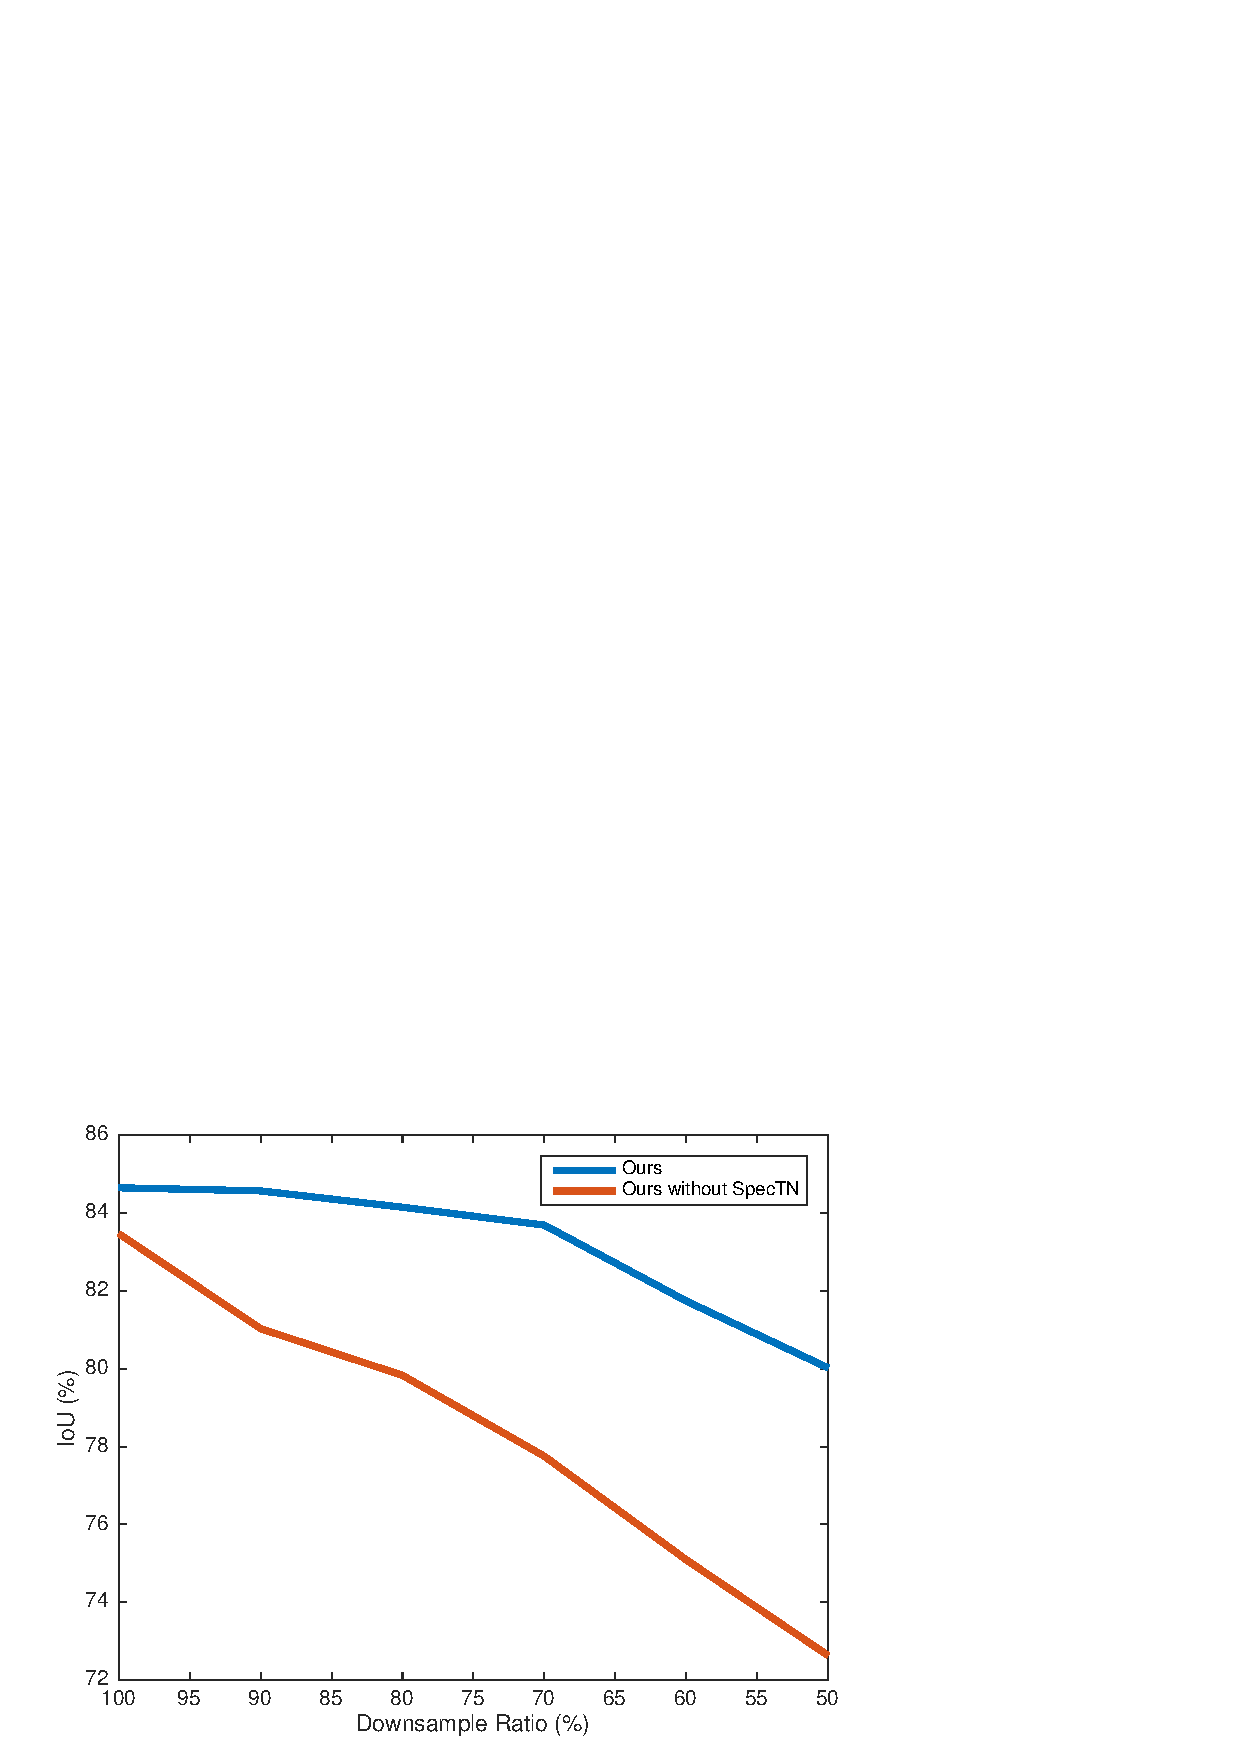
\includegraphics[width=0.8\linewidth]{./fig/downsample.pdf}
 \caption{We evaluate the robustness of our model to sampling density change. Test shapes are downsampled by different ratios and fed into our network. We compute the segmentation IoU for different downsample ratios and show it here. With SpecTN, our framework becomes more robust to sampling density change.}
 \label{fig:downsample}
\end{figure}

%\todo{Visualize joint basis}

\subsection{Qualitative Results and Error Analysis}
Figure~\ref{fig:erroranalysis} shows segmentation results generated from our network on two categories, Chair and Lamp. Representative good results are shown in the first block and  typical error patterns are summarized from the second to fourth blocks.

Most of our segmentation is very close to ground truth as is shown in the first block. We can accurately segment shapes with large geometric or topological variations like wide bench v.s. ordinary chair, pendant lamp v.s. table lamp. The lamp base on the first row and the lampshade on the second row are very similar regarding their local geometry; however, since our network is able to capture large scale context information, it could still differentiate the two and segment shapes correctly.

We observe several typical error patterns in our results. Most segmentation error occurs along part boundaries. %Our network sometimes generates fuzzy part boundaries, especially if the underlying part segments have a very smooth normal transition, as is shown in the second row of the second block. 
There are also cases where the semantic definition of parts has inherent ambiguities. %In these cases, our network may generate predictions slightly different from the ground truth but are still reasonable. 
We also observe a third type of error pattern, in which our prediction might miss a certain part completely, as is shown in the fourth block.

\begin{figure}
    \centering
    \includegraphics[width=\linewidth]{./fig/erroranalysis4.pdf}
    \caption{We visualize some segmentation results from our network prediction. The first block shows typical correct segmentations, notice the huge shape variation we can cover. The second to fourth blocks summarize different error patterns we observe in the results.}
    \label{fig:erroranalysis}
\end{figure}

\iffalse
\todo{
Compare different alternatives of our method
\begin{itemize}
    \item with multiple representatives instead of a single canonical space for spectral synchronization
    \item without join basis learning, visualize joint basis
    \item without dilated kernel, visualize dilated kernel
    \item different kernel choice: polynomial, cubic splines, exponential window, modulated exponential window
    \item different input vertex functions, extrinsic vertex functions help much since it's essentially a combination between extrinsic and intrinsic information for segmentation. intrinsic feature might not help much since the network is intrinsic and captures quite a lot intrinsic information already.
    \item network design, with/without skip link
\end{itemize}
}
\fi

\vspace{-.11in}
\paragraph{Acknowledgement}
The authors wish to thank the support of Nuro Inc., ONR MURI grant N00014-13-1-0341, NSF grants DMS-1546206 and  IIS-1528025, a Samsung GRO award, and gifts from Adobe, Amazon, and Apple.

% \section{Conclusion}
% \section{Conclusion}\label{sec:conclusion}
%\vspace{-.1in}
In this work, we apply the attentional encoder-decoder for the task of abstractive summarization with very promising results, outperforming state-of-the-art results significantly on two different datasets. Each of our proposed novel models addresses a specific problem in abstractive summarization, yielding further improvement in performance. We also propose a new dataset for multi-sentence summarization and establish benchmark numbers on it. As part of our future work, we plan to focus our efforts on this data and build more robust models for summaries consisting of multiple sentences.


%Our results strongly demonstrate that sequence-to-sequence models are extremely promising for summarization. Some of the other lessons we learned from our experiments are: (i) the LVT-trick is very useful for summarization as it improves training speed while not sacrificing performance; (ii) traditional methods such as vocabulary expansion and syntax-based features can boost performance of deep learning based models as well. As part of our ongoing work, we are investigating on ways to effectively generate rare words in the summary, which appears to be a glaring weakness in the existing models.  


\newpage
{\small
\bibliographystyle{ieee}
\bibliography{pcl}
}

\newpage
\section{Model Architecture}
\label{sec:model_detail}

\subsection{Architectural Choices}

The proposed scheme in Section~\ref{sec:main} is a general framework where one
can freely define, for instance, the activation functions $f$ of recurrent
neural networks (RNN) and the alignment model $a$. Here, we describe the
choices we made for the experiments in this paper. 

\subsubsection{Recurrent Neural Network}
\label{sec:gatedrnn}

For the activation function $f$ of an RNN, we use the gated hidden unit
recently proposed by \citet{Cho2014}. The gated hidden unit is an alternative
to the conventional {\it simple} units such as an element-wise $\tanh$.  This
gated unit is similar to a long short-term memory (LSTM) unit proposed earlier
by \citet{Hochreiter+Schmidhuber-1997}, sharing with it the ability to better
model and learn long-term dependencies. This is made possible by having
computation paths in the unfolded RNN for which the product of derivatives is
close to 1.  These paths allow gradients to flow backward easily without
suffering too much from the vanishing
effect~\citep{Hochreiter91,Bengio-trnn93,Pascanu+al-ICML2013-small}. It is
therefore possible to use LSTM units instead of the gated hidden unit described
here, as was done in a similar context by \citet{Sutskever2014}.

The new state $s_i$ of the RNN employing $n$ gated hidden units\footnote{
    Here, we show the formula of the decoder. The same formula can be used in
    the encoder by simply ignoring the context vector $c_i$ and the related
    terms.
}
is computed by
\begin{align*}
    s_i = f(s_{i-1}, y_{i-1}, c_i) = (1 - z_i) \circ s_{i-1} + z_i \circ \tilde{s}_{i},
\end{align*}
where $\circ$ is an element-wise multiplication, and $z_i$ is the output of the
update gates (see below). The proposed updated state $\tilde{s}_{i}$ is computed
by
\begin{align*}
    \tilde{s}_{i} = \tanh \left( W e(y_{i - 1}) + U \left[ r_i \circ s_{i - 1} \right] +
    C c_i \right),
\end{align*}
where $e(y_{i-1}) \in \RR^{m}$ is an $m$-dimensional embedding of a word
$y_{i-1}$, and $r_i$ is the output of the reset gates (see below).  When $y_i$
is represented as a $1$-of-$K$ vector, $e(y_i)$ is simply a column of an
embedding matrix $E \in \RR^{m \times K}$. Whenever possible, we omit bias terms
to make the equations less cluttered.

The update gates $z_i$ allow each hidden unit to maintain its previous
activation, and the reset gates $r_i$ control how much and what information from
the previous state should be reset. We compute them by
\begin{align*}
    z_i &= \sigma \left( W_{z} e(y_{i - 1}) + U_{z} s_{i - 1} + C_{z} c_i\right), \\
    r_i &= \sigma \left( W_{r} e(y_{i - 1}) + U_{r} s_{i - 1} + C_{r} c_i\right),
\end{align*}
where $\sigma\left(\cdot\right)$ is a logistic sigmoid function.

At each step of the decoder, we compute the output probability
(Eq.~\eqref{eq:generate_y}) as a multi-layered function~\citep{Pascanu2014rec}.
We use a single hidden layer of maxout units~\citep{Goodfellow2013} and
normalize the output probabilities (one for each word) with a softmax function
(see Eq.~\eqref{eq:annotation_weight}).

\subsubsection{Alignment Model}

The alignment model should be designed considering that the model needs to be
evaluated $T_x \times T_y$ times for each sentence pair of lengths $T_x$ and
$T_y$. In order to reduce computation, we use a single-layer multilayer
perceptron such that 
\begin{align*}
    a(s_{i-1}, h_j) = v_a^{\top} \tanh\left( W_a s_{i-1} + U_a h_j \right),
\end{align*}
where $W_a \in \RR^{n\times n}, U_a \in \RR^{n\times 2n}$ and $v_a \in \RR^{n}$
are the weight matrices. Since $U_a h_j$ does not depend on $i$, we can
pre-compute it in advance to minimize the computational cost. 


\subsection{Detailed Description of the Model}
\subsubsection{Encoder}

In this section, we describe in detail the architecture of the proposed model
(RNNsearch) used in the experiments (see
Sec.~\ref{sec:exp_settings}--\ref{sec:exp_results}).  From here on, we omit all
bias terms in order to increase readability.

The model takes a source sentence of 1-of-K coded word vectors as input
\[
    \vx = (x_1, \ldots, x_{T_x}),\mbox{ }x_i \in \mathbb{R}^{K_x}
\]
and outputs a translated sentence of 1-of-K coded word vectors
\[
    \vy = (y_1, \ldots, y_{T_y}),\mbox{ }y_i \in \mathbb{R}^{K_y},
\]
where $K_x$ and $K_y$ are the vocabulary sizes of source and target languages,
respectively. $T_x$ and $T_y$ respectively denote the lengths of source and
target sentences.

First, the forward states of the bidirectional recurrent neural network (BiRNN)
are computed:
\begin{align*}
    \ora{h}_i =& 
    \begin{cases}
        (1 - \ora{z}_i) \circ \ora{h}_{i-1}  + \ora{z}_i \circ \ora{\underline{h}}_{i} &\mbox{, if }i > 0 \\
        0 &\mbox{, if }i = 0
    \end{cases}
\end{align*}
where
\begin{align*}
    \ora{\underline{h}}_i =& \tanh \left( \ora{W} \ov{E} x_i + \ora{U}\left[ \ora{r}_i \circ \ora{h}_{i-1} \right] \right) \\
    \ora{z}_i =& \sigma\left( \ora{W}_z \ov{E} x_i + \ora{U}_z \ora{h}_{i-1} \right) \\
    \ora{r}_i =& \sigma\left( \ora{W}_r \ov{E} x_i + \ora{U}_r \ora{h}_{i-1} \right).
\end{align*}
$\overline{E} \in \mathbb{R}^{m\times K_x}$ is the word embedding matrix.
$\ora{W}, \ora{W}_z, \ora{W}_r \in \mathbb{R}^{n\times m}$, $\ora{U}, \ora{U}_z,
\ora{U}_r \in \mathbb{R}^{n\times n}$ are weight matrices. $m$ and $n$ are the word
embedding dimensionality and the number of hidden units, respectively. 
$\sigma(\cdot)$ is as usual a logistic sigmoid function.

The backward states $(\ola{h}_1, \cdots, \ola{h}_{T_x})$ are computed similarly.
We share the word embedding matrix $\ov{E}$ between the forward and backward
RNNs, unlike the weight matrices.

We concatenate the forward and backward states to to obtain the annotations
$(h_1, h_2, \cdots, h_{T_x})$, where
\begin{align}
    \label{eq:annotation}
    h_i = \left[ 
        \begin{array}{c}
    \ora{h}_i \\
    \ola{h}_i 
\end{array}
\right]
    \end{align}

\subsubsection{Decoder}

The hidden state $s_i$ of the decoder given the annotations from the encoder is
computed by
\begin{align*}
    s_i =& (1 - z_i) \circ s_{i-1} + z_i \circ \tilde{s}_i,
\end{align*}
where
\begin{align*}
    \tilde{s}_{i} =& \tanh \left( W E y_{i - 1} + U \left[ r_i \circ s_{i - 1} \right] +
    C c_i \right) \\ 
    z_i =& \sigma\left( W_z E y_{i - 1} + U_z s_{i-1} 
    + C_z c_i \right)\\
    r_i =& \sigma\left( W_r E y_{i - 1} + U_r s_{i-1}
    + C_r c_i \right)
\end{align*}
$E$ is the word embedding matrix for the target language.
$W, W_z, W_r \in \mathbb{R}^{n\times m}$, 
$U, U_z, U_r \in \mathbb{R}^{n\times n}$, and
$C, C_z, C_r \in \mathbb{R}^{n\times 2n}$ are weights. Again, $m$ and $n$ are the word
embedding dimensionality and the number of hidden units, respectively.
The initial hidden state $s_0$ is computed by 
$
    s_{0} = \tanh\left( W_s \ola{h}_1 \right),
$
where $W_s \in \RR^{n \times n}$.

The context vector $c_i$ are recomputed at each step by the alignment model:
\begin{align*}
    c_i =& \sum_{j=1}^{T_x} \alpha_{ij} h_j,
\end{align*}
where
\begin{align*}
    \alpha_{ij} =& \frac{\exp\left(e_{ij}\right)}{\sum_{k=1}^{T_x}
    \exp\left(e_{ik}\right)}  \\
    e_{ij} =& v_a^{\top} \tanh\left( W_a s_{i-1} + U_a h_j \right),
\end{align*}
and $h_j$ is the $j$-th annotation in the source sentence (see
Eq.~\eqref{eq:annotation}).  $v_a \in \mathbb{R}^{n'}, W_a \in
\mathbb{R}^{n'\times n}$ and $U_a \in \mathbb{R}^{n'\times  2n}$ are weight
matrices.  Note that the model becomes
RNN Encoder--Decoder~\citep{Cho2014}, if we fix $c_i$ to $\ora{h}_{T_x}$.

With the decoder state $s_{i-1}$, the context $c_{i}$ and the last generated word
$y_{i-1}$, we define the probability of a target word $y_{i}$ as
\begin{align*}
    p(y_{i}|s_i,y_{i-1},c_{i}) \propto& \exp\left(y_{i}^{\top} W_o t_{i}\right),
\end{align*}
where
\begin{align*}
    t_i =&  \left[ \max\left\{\tilde{t}_{i, 2j-1}, \tilde{t}_{i,2j}\right\}
    \right]_{j=1,\ldots,l}^{\top}
\end{align*}
and $\tilde{t}_{i,k}$ is the $k$-th element of a vector $\tilde{t}_i$ which is
computed by
\begin{align*}
    \tilde{t}_{i} =& U_o s_{i - 1} + V_o E y_{i-1} + C_o c_i.
\end{align*}
$W_o \in \mathbb{R}^{K_y\times  l}$, $U_o \in \mathbb{R}^{2l\times n}$, $V_o \in
\mathbb{R}^{2l\times m}$ and $C_o \in \mathbb{R}^{2l\times 2n}$ are weight
matrices. This can be understood as having a deep output~\citep{Pascanu2014rec}
with a single maxout hidden layer~\citep{Goodfellow2013}.

\subsubsection{Model Size}

For all the models used in this paper, the size of a hidden layer $n$ is 1000,
the word embedding dimensionality $m$ is 620 and the size of the maxout hidden
layer in the deep output $l$ is 500. The number of hidden units in the alignment
model $n'$ is 1000.

\begin{table}[t]
    \centering                                                                                         
    \begin{tabular}{c|cccccc}                                                                           
        Model & Updates {\scriptsize ($\times 10^5$)} & Epochs 
        & Hours & GPU & Train NLL & Dev. NLL \\
        \hline                                                           
        \hline
        RNNenc-30 & 8.46 & 6.4 & 109 & {\small TITAN BLACK} & 28.1 & 53.0 \\                                                
        RNNenc-50 & 6.00 & 4.5 & 108 & {\small Quadro K-6000} & 44.0 & 43.6 \\
        \hline
        RNNsearch-30 & 4.71 & 3.6 & 113 & {\small TITAN BLACK} & 26.7 & 47.2 \\
        RNNsearch-50 & 2.88 & 2.2 & 111 & {\small Quadro K-6000} & 40.7 & 38.1 \\
        \hline
    RNNsearch-50$^\star$ & 6.67 & 5.0 & 252 & {\small Quadro K-6000} & 36.7 & 35.2 \\
    \end{tabular}                                                                                      
    \caption{Learning statistics and relevant information. Each update
        corresponds to updating the parameters once using a single minibatch. 
        One epoch is one pass through the training set.
        NLL is the average conditional log-probabilities of the
        sentences in either the training set or the development set. Note that
    the lengths of the sentences differ.}
    \label{tbl:stat}                                                                                   
\end{table}                                                                                            


\section{Training Procedure}
\label{sec:training_detail}

\subsection{Parameter Initialization}

We initialized the recurrent weight matrices $U, U_z, U_r, \ola{U}, \ola{U}_z,
\ola{U}_r, \ora{U}, \ora{U}_z$ and $\ora{U}_r$ as random orthogonal matrices.
For $W_a$ and $U_a$, we initialized them by sampling each element from the
Gaussian distribution of mean $0$ and variance $0.001^2$. All the elements of
$V_a$ and all the bias vectors were initialized to zero. Any other weight matrix
was initialized by sampling from the Gaussian distribution of mean $0$ and
variance $0.01^2$.

\subsection{Training}

We used the stochastic gradient descent (SGD) algorithm.
Adadelta~\citep{Zeiler2012} was used to automatically adapt the learning rate of
each parameter ($\epsilon=10^{-6}$ and $\rho=0.95$). We explicitly normalized
the $L_2$-norm of the gradient of the cost function each time to be at most a
predefined threshold of $1$, when the norm was larger than the
threshold~\citep{Pascanu2013}.  Each SGD update direction was computed with a
minibatch of 80 sentences. 

At each update our implementation requires time proportional to the length of
the longest sentence in a minibatch. Hence, to minimize the waste of
computation, before every 20-th update, we retrieved 1600 sentence pairs, sorted them
according to the lengths and split them into 20 minibatches. The training data
was shuffled once before training and was traversed sequentially in this manner.

In Tables~\ref{tbl:stat} we present the statistics related to training all the
models used in the experiments.


\section{Translations of Long Sentences}
\label{sec:long_translation}

\begin{table}[htp]
    \begin{minipage}{0.99\textwidth}
        \small
        \centering
        \begin{tabular}{p{1.9cm} | p{12cm}}
%Source & Everything can't be sorted out in one appointment, but you know you can count on the psychiatrist, call on him if needed, that you have not been abandoned to yourself.
%\\
%\hline Reference & Ce n'est pas une s\'eance qui fait tout mais on sait qu'on peut compter sur lui, le rappeler si besoin, qu'on n'est pas livr\'es à nous-m\^emes.
%\\
%\hline RNNenc-50 & Tout ne peut pas \^etre inscrit dans une nomination, mais vous savez que vous pouvez compter sur le psychiatre, si vous le d\'esirez, si vous n'avez pas \'et\'e abandonn\'es.
%\\
%\hline RNNsearch-50 & Tout ne peut pas \^etre r\'egl\'e par une nomination, mais vous savez que vous pouvez compter sur le psychiatre, qu'il vous demande si cela est n\'ecessaire, que vous n'avez pas \'et\'e abandonn\'e.
%\\
%\hline Google \mbox{Translate} & Tout ne peut pas \^etre rgl en un seul rendez-vous, mais
%vous savez que vous pouvez compter sur le psychiatre, faire appel à lui en cas
%de besoin, que vous n'avez pas t abandonn à vous-m\^eme.
%\\
%\hline
%\multicolumn{2}{c}{} \\
\hline Source & An admitting privilege is the right of a doctor to admit a patient to a hospital or a medical centre to carry out a diagnosis or a procedure, based on his status as a health care worker at a hospital.
\\
\hline Reference & Le privilège d'admission est le droit d'un m\'edecin, en vertu de son statut de membre soignant d'un h\^opital, d'admettre un patient dans un h\^opital ou un centre m\'edical afin d'y d\'elivrer un diagnostic ou un traitement.
\\
\hline RNNenc-50 & Un privilège d'admission est le droit d'un m\'edecin de reconnaître un patient à l'h\^opital ou un centre m\'edical d'un diagnostic ou de prendre un diagnostic en fonction de son \'etat de sant\'e.
\\
\hline RNNsearch-50 & Un privilège d'admission est le droit d'un m\'edecin d'admettre un patient à un h\^opital ou un centre m\'edical pour effectuer un diagnostic ou une proc\'edure, selon son statut de travailleur des soins de sant\'e à l'h\^opital.
\\
\hline Google \mbox{Translate} & Un privilège admettre est le droit d'un m\'edecin
d'admettre un patient dans un h\^opital ou un centre m\'edical pour effectuer un
diagnostic ou une proc\'edure, fond\'ee sur sa situation en tant que travailleur de
soins de sant\'e dans un h\^opital.
\\
\hline
\multicolumn{2}{c}{} \\
%\hline Source & For the third quarter ended September 30 , Bombardier 's net profit fell to \$ 147 million , or 8 cents per share , from \$ 172 million , or 9 cents per share a year earlier .
%\\
%\hline Reference & Au troisième trimestre clos le 30 septembre , le b\'en\'efice net de Bombardier a chut\'e à 147 M \$ , ou 8 cents par action , par rapport à 172 M \$ , ou 9 cents par action , un an plus t\^ot .
%\\
%\hline RNNenc-50 & Pour le troisième trimestre termin\'e le 30 septembre , le b\'en\'efice net de Bombardier a chut\'e de 147 milliards de dollars , soit 8 cents , soit de 172 millions de dollars , soit 9 millions de dollars par an .
%\\
%\hline RNNsearch-50 & Pour le troisième trimestre , le 30 septembre , le b\'en\'efice net de Bombardier est tomb\'e à 147 millions de dollars , soit 8 cents par action , soit de 172 millions de dollars , soit 9 cents par action par rapport à l' ann\'ee pr\'ec\'edente .
%\\
%\hline
%\multicolumn{2}{c}{} \\
\hline Source & 
This kind of experience is part of Disney's efforts to "extend
the lifetime of its series and build new relationships with audiences via
digital platforms that are becoming ever more important," he added.
\\
\hline Reference & Ce type d'exp\'erience entre dans le cadre des efforts de Disney pour "\'etendre la dur\'ee de vie de ses s\'eries et construire de nouvelles relations avec son public grâce à des plateformes num\'eriques qui sont de plus en plus importantes", a-t-il ajout\'e.
\\
\hline RNNenc-50 & Ce type d'exp\'erience fait partie des initiatives du Disney pour "prolonger la dur\'ee de vie de ses nouvelles et de d\'evelopper des liens avec les lecteurs num\'eriques qui deviennent plus complexes.
\\
\hline RNNsearch-50 & Ce genre d'exp\'erience fait partie des efforts de Disney pour "prolonger la dur\'ee de vie de ses s\'eries et cr\'eer de nouvelles relations avec des publics via des plateformes num\'eriques de plus en plus importantes", a-t-il ajout\'e.
\\
\hline Google \mbox{Translate} & Ce genre d'exp\'erience fait partie des efforts de Disney
à ``\'etendre la dur\'ee de vie de sa s\'erie et construire de nouvelles relations avec
le public par le biais des plates-formes num\'eriques qui deviennent de plus en
plus important'', at-il ajout\'e.
\\
\hline
\multicolumn{2}{c}{} \\
\hline Source & 
In a press conference on Thursday, Mr Blair stated that there was nothing in
this video that might constitute a "reasonable motive" that could lead to
criminal charges being brought against the mayor.
\\
\hline Reference & En conf\'erence de presse, jeudi, M. Blair a affirm\'e qu'il n'y avait rien dans cette vid\'eo qui puisse constituer des "motifs raisonnables" pouvant mener au d\'ep\^ot d'une accusation criminelle contre le maire.
\\
\hline RNNenc-50 & Lors de la conf\'erence de presse de jeudi, M. Blair a dit qu'il n'y avait rien dans cette vid\'eo qui pourrait constituer une "motivation raisonnable" pouvant entraîner des accusations criminelles port\'ees contre le maire.
\\
\hline RNNsearch-50 & Lors d'une conf\'erence de presse jeudi, M. Blair a d\'eclar\'e qu'il n'y avait rien dans cette vid\'eo qui pourrait constituer un "motif raisonnable" qui pourrait conduire à des accusations criminelles contre le maire.
\\
\hline Google \mbox{Translate} & 
Lors d'une conf\'erence de presse jeudi, M. Blair a d\'eclar\'e qu'il n'y avait rien
dans cette vido qui pourrait constituer un "motif raisonnable" qui pourrait
mener à des accusations criminelles portes contre le maire.
\\
\hline
        \end{tabular}
    \end{minipage}
    \caption{The translations generated by RNNenc-50 and RNNsearch-50 from long
        source sentences (30 words or more) selected from the test set. For each
        source sentence, we also show the gold-standard translation.  The
        translations by Google Translate were made on 27 August 2014.
}

\label{tab:translations}
\end{table}



\end{document}
